%
%                       This is a basic LaTeX Template
%                       for the Informatics Research Review

\documentclass[a4paper,11pt]{article}
% \usepackage[numbers]{natbib}
\usepackage{amssymb}
% \usepackage[demo]{graphicx}
\usepackage{caption}
\usepackage{subcaption}
\usepackage{svg}
\usepackage{amsmath}

\usepackage{titlesec}

\titlespacing\section{0pt}{12pt plus 4pt minus 2pt}{0pt plus 2pt minus 2pt}
\titlespacing\subsection{0pt}{12pt plus 4pt minus 2pt}{0pt plus 2pt minus 2pt}
\titlespacing\subsubsection{0pt}{12pt plus 4pt minus 2pt}{0pt plus 2pt minus 2pt}


% Add local fullpage and head macros
\usepackage{head,fullpage}     
% Add graphicx package with pdf flag (must use pdflatex)
\usepackage[pdftex]{graphicx}  
% Better support for URLs
\usepackage{url}
% Date formating
\usepackage{datetime}
% For Gantt chart
\usepackage{pgfgantt}
\usepackage{xcolor}
\usepackage[utf8]{inputenc}
\setcounter{tocdepth}{1}

\newdateformat{monthyeardate}{%
  \monthname[\THEMONTH] \THEYEAR}

\parindent=0pt          %  Switch off indent of paragraphs 
\parskip=5pt            %  Put 5pt between each paragraph  
\Urlmuskip=0mu plus 1mu %  Better line breaks for URLs


%                       This section generates a title page
%                       Edit only the following three lines
%                       providing your exam number, 
%                       the general field of study you are considering
%                       for your review, and name of IRR tutor

\let\oldthebibliography\thebibliography
\let\endoldthebibliography\endthebibliography
\renewenvironment{thebibliography}[1]{
  \begin{oldthebibliography}{#1}
    \setlength{\itemsep}{0.05em}
    \setlength{\parskip}{0.02em}
}
{
  \end{oldthebibliography}
}

% \patchcmd{\thebibliography}
%   {\settowidth}
%   {\setlength{\itemsep}{0pt plus 0.0pt}\settowidth}
%   {}{}

\newcommand{\examnumber}{s1680171}
\newcommand{\field}{Predicting wave propagation on shallow water using physics-inspired representation learning}
\newcommand{\tutor}{James Garforth}
\newcommand{\supervisor}{Amos Storkey}

\begin{document}
\begin{minipage}[b]{110mm}
        {\Huge\bf School of Informatics
        \vspace*{17mm}}
\end{minipage}
\hfill
\begin{minipage}[t]{40mm}               
        \makebox[40mm]{
        \includegraphics[width=40mm]{crest.png}}
\end{minipage}
\par\noindent
    % Centre Title, and name
\vspace*{2cm}
\begin{center}
        \Large\bf Informatics Project Proposal \\
        \vspace*{1cm}
        \Large\bf \field
\end{center}
\vspace*{1.5cm}
\begin{center}
        \bf \examnumber\\
        \monthyeardate\today
\end{center}
\vspace*{4mm}

%
%                       Insert your abstract HERE
%                       
\begin{abstract}
  Wave propagation is an important problem from both a theoretical and practical point of view because it is key to many fields of science and engineering. The current numerical solvers are slow and cannot be used in iterative design work-flows. In recent years various deep learning methods have been used to produce fast approximations but a systematic assessment is lacking as of now. This work intends to fill this gap by comparing generic frame prediction architectures to methods specialized on fluid flow in terms of accuracy, speed and generalization to other physical systems. Furthermore, we propose a new architecture that stands between generic and specialized methods, inspired by a \textcolor{red}{Hamiltonian} formulation for conservative systems aiming to provide further insights on how learning algorithms encapsulate the dynamics in physical systems. 
\end{abstract}

\vspace*{0cm}
\vspace*{2cm}
Date: \today
\vfill
{\bf Tutor:} \tutor\\
{\bf Supervisor:} \supervisor
\newpage

%                                               Through page and setup 
%                                               fancy headings
\setcounter{page}{1}                            % Set page number to 1
\footruleheight{1pt}
\headruleheight{1pt}
\lfoot{\small School of Informatics}
\lhead{Informatics Research Review}
\rhead{- \thepage}
\cfoot{}
\rfoot{Date: \date{\today}}
%
\tableofcontents                                % Makes Table of Contents

\section{Motivation}\label{sec:1motivation}

% 3.  How will/has the problem been solved?

% 4.  How is the proposed solution different/better than prior work?

% 5a. What are the results? We don't have that but your final dissertation will, so your proposal should contain a plan that is likely to lead to interesting results.

% Introduce the topic of research and explain its academic and industrial context.

% \begin{itemize}
%     \item Establish the general subject area.
%     \item Describe the broad foundations of your study -- provide adequate background for readers.
%     \item Indicate the general scope of your project.
%     \item Provide an overview of the sections that will appear in your proposal (optional).
%     \item Engage the readers.
% \end{itemize}

% \subsection{Saint Venant Equations}

% Shallow water equations. 

% $$
% \frac{\partial h} {\partial t} &+ \frac{\partial}{\partial x} \Bigl( (H+h) u \Bigr) + \frac{\partial}{\partial y} \Bigl( (H+h) v \Bigr) = 0,
% $$

% $$
% \frac{\partial u}{\partial t} &+ u\frac{\partial u}{\partial x} + v\frac{\partial u}{\partial y} - f v = -g \frac{\partial h}{\partial x} - b u + \nu \left( \frac{\partial^2 u}{\partial x^2} + \frac{\partial^2 u}{\partial y^2} \right),\\[3pt]
% $$

% $$
% \frac{\partial v}{\partial t} &+ u\frac{\partial v}{\partial x} + v\frac{\partial v}{\partial y} + f u = -g \frac{\partial h}
% {\partial y} - b v + \nu \left( \frac{\partial^2 v}{\partial x^2} + \frac{\partial^2 v}{\partial y^2} \right),
% $$
% \vskip -2mm
\subsection{Problem Statement}
% \vskip -2mm
Physical processes are characterized by gradual changes during a succession of states. Modelling such phenomena in a principled way is one of the main goals of scientific endeavour because it allows us to understand the world and predict it. Fluid flow is a physical process governed by the Navier-Stokes(N-S) equations and is found in numerous industrial applications in aerodynamics, mechanical design, bioengineering, climate modelling and computer graphics among others \cite{thuerey2018well}. N-S equations are of such importance that the Clay Mathematics Institute includes them on its Millenium Problems list, which entails a million dollars prize \cite{clay}. Analytical solutions to the N-S equation are only available in trivial cases. Instead, numerical methods like Computational Fluid Dynamics (CFD) can provide accurate approximations but come at a high computational cost \cite{ferziger2012computationalcfd}. During the process of designing a system, iteration speed is very important and faster albeit less accurate approximations are highly desirable. 

Deep learning(DL) techniques have been found able to capture efficient representations in many problems such as object detection, speech synthesis and machine translation among others \cite{lecun2015deep}. The question rises if such techniques can learn representations in physical systems such as to provide high-quality predictions with a low computational burden. This project focuses on using DL to approximate fluid flow in shallow water where there is no vertical velocity. The evolution of such a system is equivalent to wave propagation as it can be seen in Figure \ref{fig:evol}. Predicting such a problem can pave the way for approximating more complex processes. 


% \textbf{Its incompressible form is given by ∂u/∂t + u · ∇u = −1/ρ∇p + ν∇2u + g , ∇ · u = 0, where the most important quantities are flow velocity u and pressure p. The other parameters ρ, ν, g denote density, kinematic viscosity and external forces, respectively.}\textbf{The Navier-Stokes equations govern the motion of fluids and can be seen as Newton's second law of motion for fluids. The Navier-Stokes equations represent the conservation of momentum, while the continuity equation represents the conservation of mass. no viscocity gives euler equations}

\begin{figure}[ht]
\centering
\begin{center}
    
\begin{minipage}[t]{.59\linewidth}
\begin{subfigure}{.33\textwidth}
  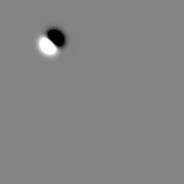
\includegraphics[width=.95\linewidth]{images/img000.jpg}
  \caption{T=0}
  \label{fig:sub1}
\end{subfigure}%
\begin{subfigure}{.33\textwidth}
  \centering
  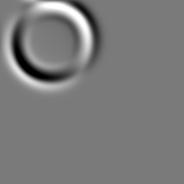
\includegraphics[width=.95\linewidth]{images/img020.jpg}
  \caption{T=20}
  \label{fig:sub2}
\end{subfigure}
\begin{subfigure}{.33\textwidth}
  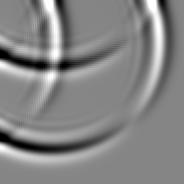
\includegraphics[width=.95\linewidth]{images/img060.jpg}
  \caption{T=60}
  \label{fig:sub3}
\end{subfigure}
\caption{Wave at different time steps T}
\label{fig:evol}
\end{minipage}
\begin{minipage}[t]{.38\linewidth}
\begin{subfigure}{.5\textwidth}
  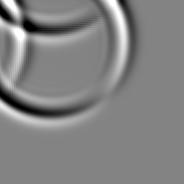
\includegraphics[width=.95\linewidth]{images/solid.jpg}
  \caption{Solid}
  \label{fig:sub1}
\end{subfigure}%
\begin{subfigure}{.5\textwidth}
  
\includegraphics[width=.95\linewidth]{images/mirror.jpg}
  \caption{Mirror}
  \label{fig:sub2}
\end{subfigure}
\caption{Boundary conditions}
\label{fig:boundary}
\end{minipage}
\end{center}

\end{figure}



\subsection{Research Hypothesis and Objectives}

% \textbf{ Cressie & Wikle (2015) also advocate the use of physical background knowledge to build statistical models.}

% \textbf{Navier–Stokes (N-S) equations need to be solved in the simulation process. Because N-S equations are nonlinear partial differential equations, many numeri- cal simulation methods, such as Lagrangian methods [1] and Eulerian methods [2,3], are used to discretize them. In the field of high-resolution fluid simulation, Eulerian methods are widely used because they are more accurate in reconstructing and rendering surface.}

Simulation methods for fluid flow are divided into two broad categories:  \textbf{Eulerian methods} which predict the velocity and pressure fields over a discrete mesh and \textbf{Langragian methods} that take into account the properties and interactions between the individual objects \cite{zhang2007comparison}. The emerging DL approximation techniques are also characterized by the same dichotomy but their qualitative and quantitative differences have not been studied extensively. It is unclear what their representations actually capture, their understanding of the process can only be measured by their predictive power. While there are success stories denoting their efficacy \cite{tompson2017accelerating} the numerical simulation community remains skeptical towards DL techniques due to their black box nature. At the same time, performance comparisons are scarce because fluid flow has too many applications and this has led to a very segmented field and a lack of commonly used datasets that would enable fair comparisons. The \textit{first objective} of this work is to compare DL techniques specifically designed for fluid flow approximation against generic video prediction methods on the same 2-d wave propagation dataset and assess their strengths and weaknesses.

We expect that specialized architectures due to higher induction bias will perform better than generic ones but also be less transferable to other problems. Our \textit{hypothesis} is that in this performance-generalization trade-off it is possible to find a hybrid approach that takes into account a narrow set of assumptions and is applicable to a wider range of physical problems. Particularly, we plan to induce a physical prior based on the law of conservation of energy which describes a multitude of physical systems. This is, to the best of our knowledge, a novel approach that if proven successful could find applications in a wide range of fields. 

The scope of this works is fast approximations of fluid flow, it does not aim to provide a substitute for numerical solutions in cases where very high accuracy is essential.

\subsection{Timeliness and Novelty}
% \vskip -2mm

 Recent years saw a lot of technological advances with the appearance of specialized GPU hardware and the parallelization of learning algorithms. This led to the resurgence of machine learning and specifically of DL which proved to be successful in many areas \cite{lecun2015deep}. The application of DL is only increasing with time as more fields adopt the new tool-sets to solve previously intractable problems. Machine learning has a long been used in CFD to aid with simulations \cite{ferziger2012computationalcfd}. The aforementioned advances can provide more accurate and fast approximations of physical phenomena in general and CFD simulations in particular. The application of DL in CFD is in its nascent phase but is growing rapidly. At this point shedding more light to how the current approaches compare will provide the consolidation that is fundamental for the advancement of any field in this stage. Furthermore, the proposed hybrid method aims to bridge the gap between current approaches and open the way for applications in a much wider spectrum of problems.

\subsection{Significance and beneficiaries}

% Navier-Stokes equations describe many phenomena of scientific and engineering interest. They are used to model ocean currents, predict the weather, design cars and aircrafts, explain flow in blood vessels, describe the dissipation of pollutants to name just a few applications. There are many domains where a trade-off between speed and accuracy can be highly desirable. For example, during an iterative design work-flow, fast and accurate enough approximations can drastically reduce the time and cost needed for each iteration. In medicine, having a faster prediction of surgery outcomes would enable better pre-operational planning. 

Overall this project will help both scientists and engineers to better understand the advantages and limitations of current DL fluid flow approximation methods. There are many applications where speed is more important than approximation accuracy. For example in iterative design work-flows, it can drastically reduce time and costs. In medicine, having a faster prediction of blood flow would enable better pre-operational planning. Furthermore, if our novel hybrid approach is proven successful this will illustrate how physics inspired methods can maintain a high level of explainability and also be practically applied. Since our assumptions are very generic, the method will be useful for the understanding of many other physical systems beyond fluid flow simulations. 

Our results will be presented to the scientific community through the final thesis and further dissemination by participating in conferences will be pursued. We are also in collaboration with groups from other Universities that are already working on the problem \cite{sorteberg2018approximating}. All the code developed during this project will become available to the community as open source.

\subsection{Feasibility}
% \vskip -2mm

Implementing and evaluating the baselines and the proposed method can be a slow process. Specifically, training can take long so we plan to run a feasibility study in order to understand how much model tweaking and development would be reasonable to do given our resources. See also relevant discussion in Section \ref{sec:3risk}. 

\vskip -6mm
\section{Background}\label{sec:2background}
% \vskip -2mm
Predicting the evolution of physical systems through machine learning became a fast-growing field with the advent of the deep learning era. As in traditional fluid flow simulations, DL techniques divided into two main categories Eulerian and Langragian \cite{zhang2007comparison}.

 From the point of view of machine learning, Langragian approaches can be thought of as either generic frame prediction or object-centric approaches as for example in intuitive physics. In the latter case, convolution-based neural networks with compositional structure can capture pairwise interactions of rigid objects and have been used to predict object movements in videos \cite{watters2017visualvin}. Graph networks extend this idea to control deformable objects consisting of nodes \cite{battaglia2018relationalgn}. In fluid dynamics, the Smoothed Particle Hydrodynamics (SPH) method approximates the N-S equations using a particle-based formulation of advection. Modelling so many particles is hard for current DL architectures, regression forests and hand-crafted features have been used to predict the velocity of each particle in the next time-step and speed-up the simulation \cite{jeong2015dataladickyforest}. 
 
 Langragian approaches in computer vision are equivalent to frame prediction where the focus shifts from object interactions to capturing the dynamics behind image changes. Estimating the optical flow field is part of many methods and relies on the assumption that surfaces are continuous over time and so the intensity of a surface remains unchanged even if its position has shifted. Deep Learning models have been used for estimating the optical flow between two frames.  FlowNet, for example, uses an autoregressive Convolutional-Deconvolutional NN (CDNN) pretrained on synthetic data to make real video prediction \cite{fischer2015flownet} but optical flow can also be estimated in an unsupervised way \cite{jason2016back} using a CNN and Long Short-Term Memory (LSTM) \cite{hochreiter1997longlstm} network. Next frame prediction using optical flow is also possible by using differentiable memory modules \cite{patraucean2015spatio}, one of our baselines, or by applying affine convolutional transformations on image parts \cite{finn2016unsupervised}. There are also approaches tailored to predict physical phenomena. In a work that will be assessed in this project, it has been shown that calculating the optical flow with a CDNN and applying a Gaussian warping scheme to enforce smoothness it is possible to predict sea surface temperature \cite{bezenac2017deep}, a transport phenomena very similar to the wave propagation that we are studying.

Frame prediction without a motion field is also possible. In their work, Mathieu et al. \cite{mathieu2015deep} use an autoregressive CDNN along with a loss that ensures sharpness and train it adversarially. Kalchbrenner et al. proposed a form of conditional autoencoder with CNN encoders, LSTM and PixelCNN predictors, producing state of the art results. With respect predicting physical systems, Convolutional LSTM \cite{xingjian2015convolutional} modules have been used to predict snow precipitation and have since been extensively applied in frame prediction being part of one the models that we will be assessing \cite{patraucean2015spatio}. Predicting Langrangian object trajectories in height fields with CNNs and RNNs has also been explored \cite{ehrhardt2017learning}. Similarly, an approximate solution to wave propagation with autoencoders and LSTM has shown promising results \cite{sorteberg2018approximating} and due to its similarity to our problem is another of our baseline models.
 
Despite that Eulerian methods are out of scope, they provide viable alternatives and can be considered for future work. In Eulerian methods during the projection step, the pressure field is calculated by solving the Poisson equation which is computationally expensive. Machine and deep learning techniques can replace numerical computations in the projection step to speed-up the simulation process. Farimani et al. \cite{farimani2017deep} have proposed using GANs conditioned on boundary conditions to infer solutions for steady flow in lid-driven cavity problems, Tompson et al. \cite{tompson2017accelerating} use domain-specific CNNs motivated by the linear system structure to speed-up the pressure projection step while Thurey et al. \cite{thuerey2018well} estimate both the pressure and velocity fields using a U-net architecture to improve flow prediction around an airfoil. The temporal evolution of the pressure field can also be modelled and used to create realistic animations of fluids \cite{wiewel2018latent}. Applications of Eulerian DL methods also extend to speeding-up Lattice Boltzmann Methods for compressible Euler equations by four orders of magnitude \cite{guo2016convolutional}, modelling turbulence for improved Reynolds stress closure \cite{ling2016reynolds} and inverse problems like shape optimization \cite{umetani2018learning}.


\section{Programme and Methodology}\label{sec:3methods}
% \vskip -2mm
% \vskip -2mm

This project focuses on two categories of frame prediction methods, generic ones and methods specifically designed for prediction of transport phenomena. While both categories share similarities, methods specifically developed for fluid flow are expected to be more accurate in modeling the shallow water wave propagation that we study but also harder to transfer to other physical processes. To further study this generalization-performance trade-off, we propose a new formulation for prediction based on the idea of energy conservation in order to target a wider spectrum of physical processes. Following we describe in detail the baselines, the proposed method, risks involved in developing the methods and also discuss some potential ethical issues.

\subsection{Baselines}
\label{sec:3baselines}
For generic video methods, there is a plethora of methods to choose from and our selection is based on reported accuracy, their capacity to adapt and extend, the availability of open source code and the similarity of the original application to ours. Overal, we plan to implement the following baselines.

% \begin{itemize}
    % \item
\textbf{Adversarially trained CDNN.} The first baseline is a state-of-the-art method that uses an autoregressive multiscale CDNN \cite{mathieu2015deep}. To overcome the blurriness inherent in these type of models when used with the $L_2$ loss, the authors propose to adversarially train the network adding a loss that preserves the sharpness. Adversarial methods are flexible in the sense that introducing a well-designed loss can have the desired results, an avenue we are willing to explore.
% \item 


\textbf{Spatial and temporal autoencoders (ConvLSTM).} The second baseline follows a different approach, using a combination of two autoencoders one for the spatial and one for the temporal domains \cite{patraucean2015spatio}. The spatial encoder and decoders are based on convolutions. The temporal module uses a ConvLSTM \cite{xingjian2015convolutional} with an optical flow predictor based on the Huber loss and a grid sampler that feeds the decoder. ConvLSTMs where originally uses in snow precipitation forecasting so this method is expected to work well in physical processes.

We also consider two more baselines specialized in predicting transport phenomena:

\textbf{Sea temperature prediction with CDNN and a physical prior.} The third baseline is a method that draws many analogies to video prediction but also incorporates a physical prior and is used to predict sea surface temperatures  \cite{bezenac2017deep}. A CDNN estimates the motion field and then a warping scheme is applied. By assuming a Gaussian warping scheme the method induces a smoothness bias, present in many physical phenomena. Given that the Green function for wave propagation might be different this leaves room for for exploring different warping schemes.

\textbf{Wave propagation prediction with autoencoder and LSTM.} The last baseline is the most relevant one because it studies the wave propagation problem and has served as an inspiration for this project \cite{sorteberg2018approximating}. A visual autoencoder is employed to compress the input frames into a latent space, then an  propagate this latent space into the future before it is decoded back to the spatial domain. 

\subsection{Proposed method}
\label{sec:3proposed}
Apart from the baselines, a novel methodology is also proposed, occupying a spot between generic video prediction and fluid-specific approaches. The aim is to come up with a formulation applicable to a variety of physical processes and not only wave propagation. Elementary principles like conservation of energy characterize every closed physical system hence inducing such a prior is a promising direction. Specifically, we draw inspiration by Hamiltonian mechanics, a mathematical formulation that predicts the trajectories of objects moving under Newtonian laws. Under the Hamiltonian formulation a system is described by the canonical coordinates $\mathbf{z} :=(\mathbf{q}, \mathbf{p})^{T}$ with $  \mathbf{q}, \mathbf{p} \in \mathbb{R}^{d}, \mathbf{z} \in \mathbb{R}^{2 d}$, where $\mathbf{q}$ and $\mathbf{p}$ correspond to the position and momentum of the objects respectively. Denoting the total energy of the system as $H(\mathbf{z})$, the equations of motion can be written in the compact form:

\begin{center}

\begin{tabularx}{\textwidth}
\vskip -7pt
$\frac{d}{d t} \mathbf{z}= \mathbf{J} \nabla_{\mathbf{z}} H(\mathbf{z})$,
    &  & 
$\mathbf{J} :=\left[ \begin{array}{cc}{0} & {+\mathbf{I}_{d}} \\ {-\mathbf{I}_{d}} & {0}\end{array}\right]$
\end{tabularx}
\end{center}
\vskip -4pt

where $\mathbf{J}$ is a canonical structure matrix but it can be generalized to be an arbitrary invertible constant skew-symmetric matrix \cite{leimkuhler_reich_2005hamiltonian}. Since $\mathbf{J}$ is skew-symmetric and invertible it can be factorized as $\mathbf{J} = \mathbf{A\Lambda A}^T$ and following some matrix calculus the Hamiltonian can be written as $\frac{d}{d t} \mathbf{z'}= \mathbf{\Lambda} \nabla_{\mathbf{z'}} H(\mathbf{z'})$ where $\mathbf{z'} = \mathbf{Az}$. We propose modelling the process with a CDNN architecture where $\nabla_{\mathbf{z'}} H(\mathbf{z'})$ is conceptually encoded by the convolutional part,  the deconvolutions correspond to applying the derivatives of the canonical quantities $\frac{d}{d t} \mathbf{z'}$ to predict the future frame. The matrix $\mathbf{\Lambda}$ plays enforces energy conservation over local regions of the frame. Simply put, it encodes the dependencies between the canonical quantities $\mathbf{q}$ and $\mathbf{p}$ and can be designed to be block diagonal, a band matrix or some other appropriate form, while its size is also an important hyperparameter of the model. A sketch graph of this architecture is given in Figure \ref{fig:arch}. Since the system is deterministic, if the Hamiltonian assumptions hold and the design of  $\mathbf{\Lambda}$ is appropriate then the network will be able to encapsulate the dynamics and produce accurate long-term predictions.

All methods will be trained in a supervised manner and the goal is to predict the next frame given a few previous frames. It has been shown that using the $L_2$ norm between the output and the ground truth does not produce good results \cite{mathieu2015deep} so we will be using the structural similarity metric (SSIM) which compares local statistics of image regions \cite{wang2004imagessim}.

% \[
% \begin{bmatrix}
%     l_{11} & l_{12} & 0 & \dots  & 0 \\
%     l_{21} & l_{22} & l_{23} & \dots  & 0 \\
%     \vdots & \vdots & \vdots & \ddots & \vdots \\
%     0 & 0 & 0 & \dots  & l_{nn}
% \end{bmatrix}
% \]

 \begin{figure}[tb]
% \vskip 5mm
\begin{center}
%   \setlength{\unitlength}{0.1\textwidth}
\begin{picture}(320, 80)
\put(0,0){\includesvg[width=0.7\columnwidth]{images/nn-2.svg}}
\put(-70,50){Input frames}
\put(70,100){$\nabla_{\mathbf{z'}} H(\mathbf{z'})$}
\put(162,95){$\mathbf{\Lambda}$}
\put(230,90){$\frac{d}{d t} \mathbf{z'}$}
\put(330,30){Prediction}

\end{picture}
\caption{The proposed architecture inspired by the Hamiltonian formulation. A multi-frame input passes through a series of convolutional layers (here only 2 depicted) that conceptually encode the partial derivatives $\nabla_{\mathbf{z'}} H(\mathbf{z'})$. The column layers in the middle are connected through the matrix $\mathbf{\Lambda}$,  how energy is locally preserved. The transformed quantities, that correspond to the derivatives of the canonical coordinates $\frac{d}{d t} \mathbf{z'}$, are used to reconstruct the predicted future frame.}
\label{fig:arch}
\end{center}
\vskip -5mm
\end{figure}

% $$
% \begin{array}{l}{\frac{\partial h}{\partial t}+\frac{\partial}{\partial x}((H+h) u)+\frac{\partial}{\partial y}((H+h) v)=0} \\ 
% {\frac{\partial u}{\partial t}+u \frac{\partial u}{\partial x}+v \frac{\partial u}{\partial y}-f v=-g \frac{\partial h}{\partial x}-b u+\nu\left(\frac{\partial^{2} u}{\partial x^{2}}+\frac{\partial^{2} u}{\partial y^{2}}\right)} \\ 
% {\frac{\partial v}{\partial t}+u \frac{\partial v}{\partial x}+v \frac{\partial v}{\partial y}+f u=-g \frac{\partial h}{\partial y}-b v+\nu\left(\frac{\partial^{2} v}{\partial x^{2}}+\frac{\partial^{2} v}{\partial y^{2}}\right)}\end{array}
% $$
 \vskip -2mm
\subsection{Risk Assessment}
\label{sec:3risk}
% \vskip -2mm
As in any project, it is possible some aspects will not go as planned and we have taken measures to mitigate such risks. Even though we chose our baseline carefully fully implementing and adapting them to our problem and infrastructure can be tricky. Our framework of choice is \textit{pytorch} so we chose baselines for which we have access to at least one implementation either in \textit{pytorch} or \textit{tensorflow} to make the initial development easier. Furthermore, to make sure we will have a baseline that works reasonably well we plan to start with methods specific to fluids like \cite{sorteberg2018approximating} and then move to the rest. 

 Iterating fast is important when implementing and verifying techniques. This is especially true the proposed method which is a novel approach and will possibly require a lot of experiments and fine-tuning to accurately be assessed. During the feasibility study, we will assess the training times to get an idea of how many experiments could realistically run within our time constrains. If training times are too long we plan to make development iteration faster by using a smaller dataset and/or by reducing the input dimensions. Furthermore, we have deliberately chosen baselines that facilitate adaptations. If our proposed method fails to provide comparable performance we plan to try variations of our baselines as explained in Section \ref{sec:3baselines}. Lastly, having noticed from other assignments that the GPU clustered is usually over-utilized close to deadlines we plan to start the experiments as soon as possible and we have started the data-collection process already. 

\vskip -2mm
\subsection{Ethics}
\label{sec:3ethics}
During this research we follow the guidelines of the University of Edinburgh ethics policy and ensure that all sources are acknowledged. We are using synthetic datasets and planning to use open source code with the appropriate attribution. Even though solving the wave propagation problem does not raise any immediate ethical concerns, the approximate solutions  considered in this project should only be used when appropriate. To verify and test final designs of critical systems like aircrafts etc. it is important to use high-accuracy numerical solutions.

% \begin{itemize}
%     \item Detail the methodology to be used in pursuit of the research and justify this choice.
%     \item Describe your contributions and novelty and where you
%     will go beyond the state-of-the-art (new methods, new tools,
%     new data, new insights, new proofs,...)
%     \item Describe the programme of work, indicating the research to be undertaken and the milestones that can be used to measure its progress.
%     \item Where suitable define work packages and define the dependences
%     between these work packages. WPs and their dependences should be
%     shown in the Gantt chart in the research plan.
%     \item Explain how the project will be managed.
%     \item State the limitations of your research.
% \end{itemize}


% \begin{figure}
% \centering
% \begin{minipage}{.5\textwidth}
%   \centering
%   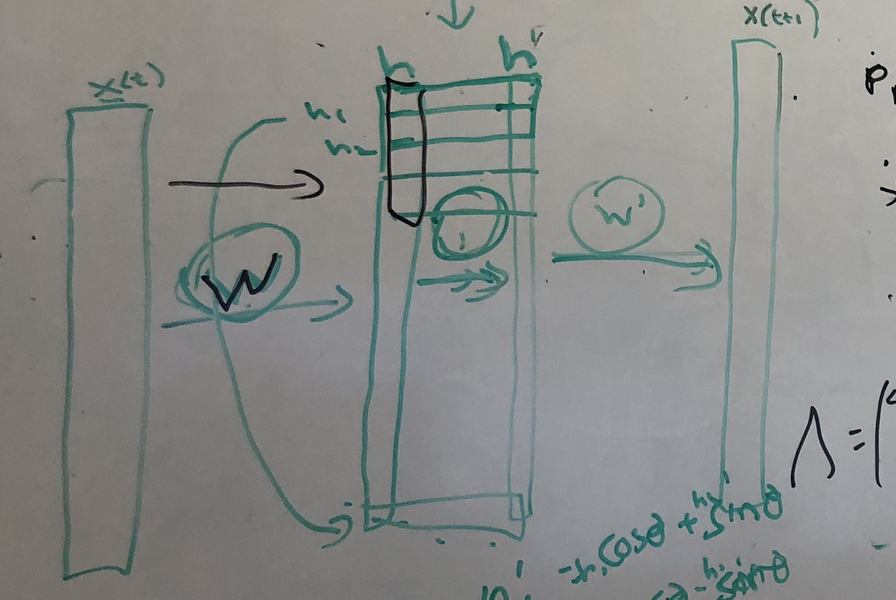
\includegraphics[width=.4\linewidth]{images/proposed.png}
%   \captionof{figure}{A figure}
%   \label{fig:test1}
% \end{minipage}%
% \begin{minipage}{.5\textwidth}
%   \centering
%   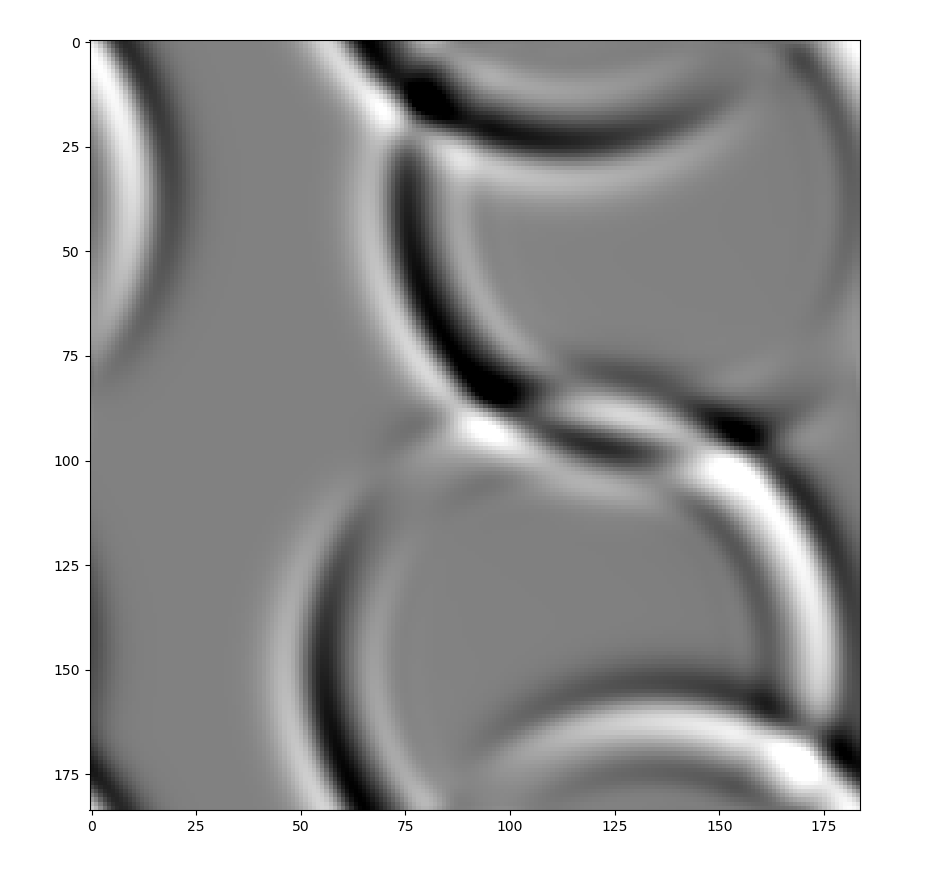
\includegraphics[width=.4\linewidth]{images/mirror.png}
%   \captionof{figure}{Another figure}
%   \label{fig:test2}
% \end{minipage}
% \end{figure}

\section{Evaluation}\label{sec:4evaluation}

% \begin{figure}[tb]
% \vskip 5mm
% \begin{center}
% \centerline{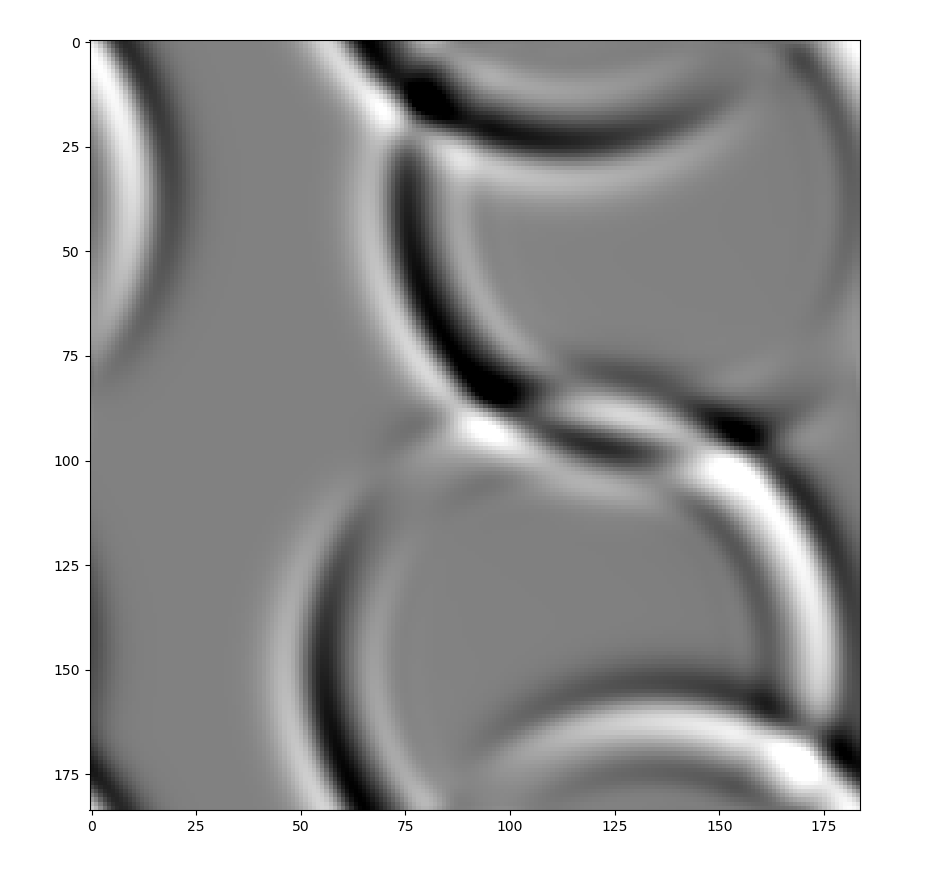
\includegraphics[width=0.3\columnwidth]{images/mirror.png}}
% \caption{Mirror Boundaries}
% \label{Decision_Boundaries}
% \end{center}
% \vskip -5mm
% \end{figure}

The methods discussed in Section \ref{sec:3methods} will be assessed on an artificial dataset that we will create using the Triflow simulator package \cite{CELLIER_2018triflow}. SSIM will be used as a metric to assess how good the prediction is relative to the ground truth future frame. We would like to assess if the networks encapsulate an intrinsic physical understanding or just spatiotemporal correlations between the pixels. Here we explain a few directions towards this goal. Long term prediction is very important, the methods will be evaluated not only on the next frame but also in subsequent ones by recursively feeding the prediction back to the network. A model should also be invariant to boundary conditions. We will try two different boundary conditions: \textit{mirror boundary}, where waves cross from one side of the frame to the other, and \textit{solid boundary}, where the waves reflect back at the boundaries as seen in Figure \ref{fig:boundary} (a) and (b) respectively. Additionally, changing the dynamics, like the depth of the water or the angle of the illumination, produces qualitatively different patterns and our models will be assessed upon how well they can generalize in those situations. The generalizations capabilities can also be determined on totally different physical prediction problems like for example a double swinging pendulum. Lastly, since our focus is on fast approximations, the time it takes to train each network along with the speed of prediction at test time are important evaluation metrics.

\vskip -10mm

\section{Expected Outcomes}\label{sec:5outcomes}

How much prior physical knowledge does machine learning require to predict physical systems well? What is the best way to incorporate it? This project will provide a comprehensive study of DL methods assessed on the wave propagation problem. We aim to shed light on the trade-offs between generic frame prediction methods and those specifically designed to estimates transport phenomena. Furthermore, we propose a new method that stands somewhere in between by targeting physical processes in general, hoping that this new method will provide another option in the wide spectrum of possibilities and better inform future research in the area.

% \textcolor{red}{How much prior physical knowledge does machine learning require to predict physical systems well? What is the best way to incorporate it? This project will provide a comprehensive study of DL methods for fluid flow. We aim to shed light on the trade-offs between generic frame methods and those specifically designed to estimates fluid flow. Furthermore, we propose a new method that stands somewhere in between by focusing on physical systems in general and hope that this new method will provide another option in the wide spectrum of possibilities and better inform future research in the area.How much prior physical knowledge does machine learning require to predict physical systems well? What is the best way to incorporate it? This project will provide a comprehensive study of DL methods for fluid flow. We aim to shed light on the trade-offs between generic frame methods and those specifically designed to estimates fluid flow.}

\section{Research Plan, Milestones and Deliverables}\label{sec:6plan}
\vskip -10mm

\definecolor{barblue}{RGB}{153,204,254}
\definecolor{groupblue}{RGB}{51,102,254}
\definecolor{linkred}{RGB}{165,0,33} 

\begin{figure}[htbp]
\begin{ganttchart}[
    y unit title=0.4cm,
    y unit chart=0.5cm,
    vgrid,hgrid,
    x unit=1.55mm,
    time slot format=isodate,
    title/.append style={draw=none, fill=barblue},
    title label font=\sffamily\bfseries\color{white},
    title label node/.append style={below=-1.6ex},
    title left shift=.05,
    title right shift=-.05,
    title height=1,
    bar/.append style={draw=none, fill=groupblue},
    bar height=.6,
    bar label font=\normalsize\color{black!50},
    group right shift=0,
    group top shift=.6,
    group height=.3,
    group peaks height=.2,
    bar incomplete/.append style={fill=green}
   ]{2018-06-01}{2018-08-16}
   \gantttitlecalendar{month=name}\\
   \ganttbar[
    progress=40,
    bar progress label font=\small\color{barblue},
    bar progress label node/.append style={right=4pt},
    bar label font=\normalsize\color{barblue},
    name=bg
   ]{Background Reading}{2018-06-01}{2018-06-14} \\
\ganttset{progress label text={}, link/.style={black, -to}}
\ganttgroup{Preliminary work}{2018-06-07}{2018-06-21} \\
\ganttbar[progress=60, name=dataset]{Dataset creation}{2018-06-07}{2018-06-14} \\
\ganttlinkedbar[progress=5, name=feasibility]{Feasibility study}{2018-06-14}{2018-06-21} \\
\ganttgroup{Model implementation}{2018-06-21}{2018-07-21} \\
\ganttbar[progress=10, name=baseline]{Baselines}{2018-06-21}{2018-07-07} \\
\ganttlinkedbar[progress=0, name=proposed]{Proposed method}{2018-07-07}{2018-07-21} \\
\ganttgroup{Dissertation}{2018-07-14}{2018-08-16} \\
  \ganttbar[progress=0, name = draft]{Draft}{2018-07-14}{2018-07-31}\\
  \ganttlinkedbar[progress=0, name = thesis]{Final thesis}{2018-08-01}{2018-08-16}
  \ganttset{link/.style={green}}
%   \ganttlink[link mid=.4]{bg}{dataset}
  \ganttlink[link mid=.4]{feasibility}{baseline}
    \ganttlink[link mid=.4]{baseline}{draft}
%         \ganttlink[link mid=.159]{draft}{thesis}
\end{ganttchart}
\caption{Gantt Chart of the activities defined for this project.}
\label{fig:gantt}
\end{figure}

\begin{table}[htbp]
    \begin{center}
        \begin{tabular}{|c|c|l|}
        \hline
        \textbf{Milestone} & \textbf{Week} & \textbf{Description} \\
        \hline
        $M_1$ & 2 & Dataset acquisition \& Feasibility study completed \\
        $M_2$ & 5 & Baselines established and evaluated \\
        $M_3$ & 7 & Proposed method implementation \& evaluation completed \\
        $M_4$ & 8 & Draft version of dissertation completed \\
        $M_5$ & 10 & Submission of dissertation \\
        \hline
        \end{tabular} 
    \end{center}
    \caption{Milestones defined in this project.}
    \label{fig:milestones}
\end{table}

\begin{table}[htbp]
    \begin{center}
        \begin{tabular}{|c|c|l|}
        \hline
        \textbf{Deliverable} & \textbf{Week} & \textbf{Description} \\
        \hline
        $D_1$ & 3 & Code base for baselines \\
        $D_2$ & 6 & Code base for proposed method and results \\
        $D_3$ & 8 & Dissertation draft \\
        $D_4$ & 10 & Final dissertation \\
        \hline
        \end{tabular} 
    \end{center}
    \caption{List of deliverables defined in this project.}
    \label{fig:deliverables}
\end{table}
\vskip -20mm
\bibliographystyle{unsrt}   % The reference style
%                This is plain and unsorted, so in the order
%                they appear in the document.

{
% \small
\footnotesize
\bibliography{main}       % bib file(s).
}
\end{document}

